%! TEX root = ../main.tex
\chapter{Work to be Done}
\label{ch:work_to_be_done}
\label{Ch_6_Work to be done}

\section{Introduction}
This chapter outlines the remaining development, integration, and validation tasks for the completion of the Autonomous Mobile Robot (AMR) project. The proposed schedule is divided into four targeted phases: foundational platform and navigation setup (Phase~1), operational telemetry and cloud dashboard integration (Phase~2), natural language goal translation and closed-loop dispatch (Phase~3), and comprehensive system validation (Testing).

\section{Planned Work}
The remaining engineering work is structured into eleven specific work packages across four distinct project phases:

\subsection*{Phase 1: Autonomous Navigation and Platform Setup}
\begin{itemize}
    \item \textbf{T1.1 --- Chassis Assembly \& Motor Driver Setup:} Complete structural fabrication and mechanical assembly. The structural platform utilizes a 6\,mm ABS lower base plate printed at 15\% infill for chassis rigidity, a 4\,mm PLA upper deck printed at 10\% infill to minimize upper-deck inertia, and solid 100\% infill ABS motor-to-wheel shaft couplers to withstand high torsional loads from the Mecanum wheels. Wire all drive motors to the motor drivers and configure low-level directional actuation and PWM velocity control.
    \item \textbf{T1.2 --- Sensor Integration (LiDAR/Camera \& Microcontroller):} Interface the perception and inertial sensors (LiDAR/cameras, MPU-6050 IMU, and ultrasonic rangefinder) with the onboard compute and microcontroller platforms.
    \item \textbf{T1.3 --- SLAM Environment Mapping \& Costmaps:} Execute exploratory indoor runs to generate high-resolution occupancy grid maps, configure inflation layers, and establish dynamic local/global costmaps.
    \item \textbf{T1.4 --- Path Planner Tuning \& Avoidance:} Tune global path planning ($A^*$/NavFn) and local trajectory optimization controllers for reliable dynamic obstacle avoidance.
\end{itemize}

\subsection*{Phase 2: Telemetry and Dashboard Infrastructure}
\begin{itemize}
    \item \textbf{T2.1 --- Sensor Telemetry Extraction (Voltage/Speed):} Implement onboard background daemons to sample battery supply voltage, wheel encoder velocities, and system health metrics at high frequency.
    \item \textbf{T2.2 --- MQTT / Wireless Communication Bridge:} Establish an event-driven pub/sub messaging bridge over Wi-Fi to serialize and stream telemetry packets asynchronously without blocking real-time motion control.
    \item \textbf{T2.3 --- DAS Database Server Setup:} Deploy a Data Acquisition Server (DAS) database backend to ingest, log, and structure continuous runtime telemetry streams.
    \item \textbf{T2.4 --- Power BI Operational Dashboard Build:} Construct an interactive, browser-accessible Power BI dashboard providing remote supervisors with real-time visual tracking of robot speed, battery curves, and active coordinate status.
\end{itemize}

\subsection*{Phase 3: Natural Language Processing and Semantic Dispatch}
\begin{itemize}
    \item \textbf{T3.1 --- LLM API / Light NLP Pipeline Integration:} Configure a lightweight NLP and Large Language Model prompt completion pipeline to parse unstructured operator voice/text commands into structured intent and entity tags.
    \item \textbf{T3.2 --- Spatial Map Database \& Coordinate Mapping:} Construct a local topological database associating common landmark and room names with calibrated Cartesian poses $(x, y, \theta)$ on the navigation map.
    \item \textbf{T3.3 --- Goal Dispatch \& End-to-End Control Loop:} Close the high-level loop by automatically passing parsed coordinate goals into the navigation action client to initiate autonomous locomotion.
\end{itemize}

\subsection*{Testing: Verification and Academic Synthesis}
\begin{itemize}
    \item \textbf{T4.1 --- System Validation \& Report:} Perform exhaustive multi-run navigation trials, assess command translation accuracy and telemetry latency, and synthesize final documentation for the project report.
\end{itemize}

\section{Timeline}
The project timeline is organized into 5-day intervals spanning from August 1 to October 15. Table~\ref{tab:project_schedule} summarizes the task duration windows, and Fig.~\ref{fig:project_gantt} illustrates the operational Gantt chart.

\begin{table}[htbp]
\centering
\small
\caption{Detailed task breakdown and execution windows across project phases.}
\label{tab:project_schedule}
\renewcommand{\arraystretch}{1.25}
\begin{tabularx}{\textwidth}{>{\raggedright\arraybackslash}p{1.8cm} >{\raggedright\arraybackslash}p{1.4cm} >{\raggedright\arraybackslash}X >{\raggedright\arraybackslash}p{3.2cm}}
\hline
\textbf{Phase} & \textbf{Task ID} & \textbf{Task Description} & \textbf{Timeline Window} \\ \hline
\multirow{4}{*}{\textbf{Phase 1}} 
 & T1.1 & Chassis Assembly \& Motor Driver Setup & Aug 1 -- Aug 10 \\ \cline{2-4}
 & T1.2 & Sensor Integration (LiDAR/Cam \& MCU) & Aug 6 -- Aug 20 \\ \cline{2-4}
 & T1.3 & SLAM Environment Mapping \& Costmaps & Aug 16 -- Aug 30 \\ \cline{2-4}
 & T1.4 & Path Planner Tuning \& Avoidance & Aug 26 -- Sep 10 \\ \hline
\multirow{4}{*}{\textbf{Phase 2}} 
 & T2.1 & Sensor Telemetry Extraction (Voltage/Speed) & Sep 1 -- Sep 10 \\ \cline{2-4}
 & T2.2 & MQTT / Wireless Communication Bridge & Sep 6 -- Sep 20 \\ \cline{2-4}
 & T2.3 & DAS Database Server Setup & Sep 11 -- Sep 20 \\ \cline{2-4}
 & T2.4 & Power BI Operational Dashboard Build & Sep 16 -- Sep 30 \\ \hline
\multirow{3}{*}{\textbf{Phase 3}} 
 & T3.1 & LLM API / Light NLP Integration & Sep 21 -- Oct 5 \\ \cline{2-4}
 & T3.2 & Spatial Map DB \& Coordinates & Sep 26 -- Oct 10 \\ \cline{2-4}
 & T3.3 & Goal Dispatch \& Control Loop & Oct 6 -- Oct 15 \\ \hline
\textbf{Testing} 
 & T4.1 & System Validation \& Report & Oct 11 -- Oct 15 \\ \hline
\end{tabularx}
\end{table}

\begin{figure}[htbp]
\centering
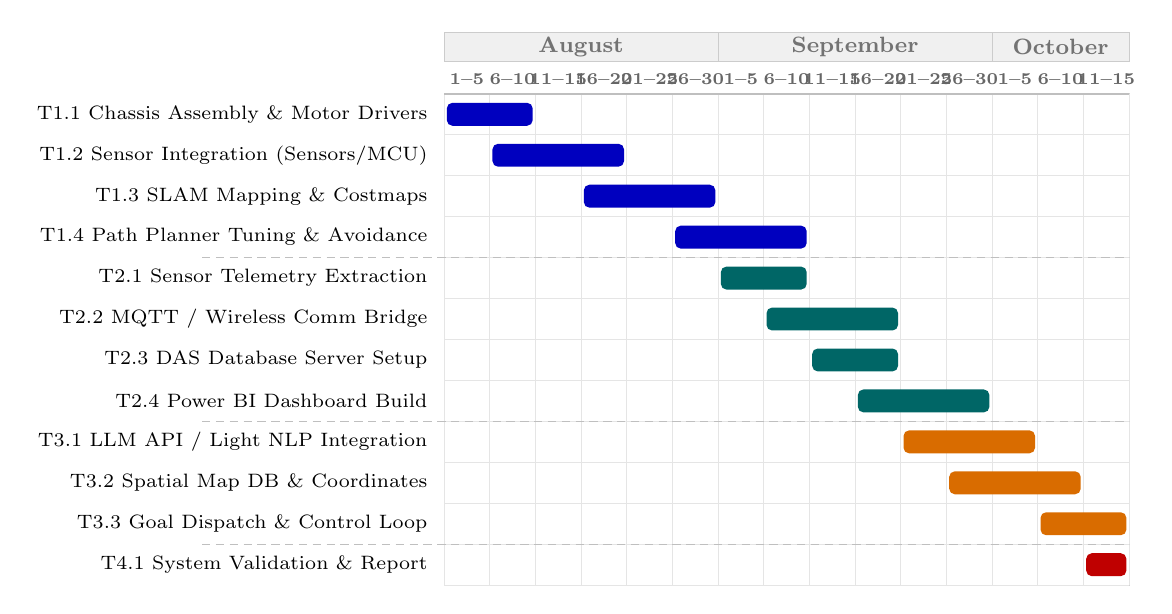
\begin{tikzpicture}[x=0.58cm, y=0.52cm]
    \draw[draw=gray!35, fill=white] (0,0) rectangle (15,12);
    \draw[help lines, color=gray!20, line width=0.35pt] (0,0) grid[xstep=1, ystep=1] (15,12);

    % Month Header Banners
    \draw[fill=gray!12, draw=gray!40, line width=0.4pt] (0, 12.8) rectangle (6, 13.5);
    \node[font=\footnotesize\bfseries, text=gray!90!black] at (3, 13.15) {August};

    \draw[fill=gray!12, draw=gray!40, line width=0.4pt] (6, 12.8) rectangle (12, 13.5);
    \node[font=\footnotesize\bfseries, text=gray!90!black] at (9, 13.15) {September};

    \draw[fill=gray!12, draw=gray!40, line width=0.4pt] (12, 12.8) rectangle (15, 13.5);
    \node[font=\footnotesize\bfseries, text=gray!90!black] at (13.5, 13.15) {October};

    % 5-Day Interval Headers
    \foreach \i/\label in {
        0.5/{1--5}, 1.5/{6--10}, 2.5/{11--15}, 3.5/{16--20}, 4.5/{21--25}, 5.5/{26--30},
        6.5/{1--5}, 7.5/{6--10}, 8.5/{11--15}, 9.5/{16--20}, 10.5/{21--25}, 11.5/{26--30},
        12.5/{1--5}, 13.5/{6--10}, 14.5/{11--15}
    } {
        \node[font=\fontsize{6}{7}\selectfont\bfseries, text=gray!80!black] at (\i, 12.35) {\label};
    }
    \draw[line width=0.5pt, color=gray!50] (0, 12) -- (15, 12);

    % Task Labels
    \node[anchor=east, font=\scriptsize] at (-0.15, 11.5) {T1.1 Chassis Assembly \& Motor Drivers};
    \node[anchor=east, font=\scriptsize] at (-0.15, 10.5) {T1.2 Sensor Integration (Sensors/MCU)};
    \node[anchor=east, font=\scriptsize] at (-0.15, 9.5) {T1.3 SLAM Mapping \& Costmaps};
    \node[anchor=east, font=\scriptsize] at (-0.15, 8.5) {T1.4 Path Planner Tuning \& Avoidance};

    \node[anchor=east, font=\scriptsize] at (-0.15, 7.5) {T2.1 Sensor Telemetry Extraction};
    \node[anchor=east, font=\scriptsize] at (-0.15, 6.5) {T2.2 MQTT / Wireless Comm Bridge};
    \node[anchor=east, font=\scriptsize] at (-0.15, 5.5) {T2.3 DAS Database Server Setup};
    \node[anchor=east, font=\scriptsize] at (-0.15, 4.5) {T2.4 Power BI Dashboard Build};

    \node[anchor=east, font=\scriptsize] at (-0.15, 3.5) {T3.1 LLM API / Light NLP Integration};
    \node[anchor=east, font=\scriptsize] at (-0.15, 2.5) {T3.2 Spatial Map DB \& Coordinates};
    \node[anchor=east, font=\scriptsize] at (-0.15, 1.5) {T3.3 Goal Dispatch \& Control Loop};

    \node[anchor=east, font=\scriptsize] at (-0.15, 0.5) {T4.1 System Validation \& Report};

    % Phase Dividing Grid Lines
    \draw[densely dashed, color=gray!50, line width=0.4pt] (-5.3, 8) -- (15, 8);
    \draw[densely dashed, color=gray!50, line width=0.4pt] (-5.3, 4) -- (15, 4);
    \draw[densely dashed, color=gray!50, line width=0.4pt] (-5.3, 1) -- (15, 1);

    % Phase 1 Bars
    \fill[rounded corners=2pt, fill=blue!75!black] (0.06, 11.22) rectangle (1.94, 11.78);
    \fill[rounded corners=2pt, fill=blue!75!black] (1.06, 10.22) rectangle (3.94, 10.78);
    \fill[rounded corners=2pt, fill=blue!75!black] (3.06, 9.22) rectangle (5.94, 9.78);
    \fill[rounded corners=2pt, fill=blue!75!black] (5.06, 8.22) rectangle (7.94, 8.78);

    % Phase 2 Bars
    \fill[rounded corners=2pt, fill=teal!80!black] (6.06, 7.22) rectangle (7.94, 7.78);
    \fill[rounded corners=2pt, fill=teal!80!black] (7.06, 6.22) rectangle (9.94, 6.78);
    \fill[rounded corners=2pt, fill=teal!80!black] (8.06, 5.22) rectangle (9.94, 5.78);
    \fill[rounded corners=2pt, fill=teal!80!black] (9.06, 4.22) rectangle (11.94, 4.78);

    % Phase 3 Bars
    \fill[rounded corners=2pt, fill=orange!85!black] (10.06, 3.22) rectangle (12.94, 3.78);
    \fill[rounded corners=2pt, fill=orange!85!black] (11.06, 2.22) rectangle (13.94, 2.78);
    \fill[rounded corners=2pt, fill=orange!85!black] (13.06, 1.22) rectangle (14.94, 1.78);

    % Testing Bar
    \fill[rounded corners=2pt, fill=red!75!black] (14.06, 0.22) rectangle (14.94, 0.78);
\end{tikzpicture}
\caption{Gantt chart illustrating the schedule and task distribution from August 1 to October 15.}
\label{fig:project_gantt}
\end{figure}

\section{Expected Outcomes}
Execution of the planned timeline will yield the following verified outcomes:
\begin{enumerate}
    \item \textbf{Autonomous Navigation Platform:} An operational AMR platform navigating dynamically within mapped environments using calibrated SLAM and obstacle costmaps.
    \item \textbf{Unified Cloud Telemetry Monitoring:} Continuous streaming of battery health, velocity vectors, and operational coordinates to a Power BI supervisory dashboard via an MQTT/wireless bridge.
    \item \textbf{Natural Language Dispatch System:} An end-to-end command interpretation loop allowing non-specialist users to dispatch spatial navigation goals via conversational text.
    \item \textbf{Comprehensive Performance Evaluation:} Documented empirical benchmarks detailing path tracking repeatability, telemetry latency, and obstacle avoidance response.
\end{enumerate}